\documentclass{ximera}

%\usepackage{todonotes}

\newcommand{\todo}{}

\usepackage{esint} % for \oiint
\graphicspath{
  {./}
  {ximeraTutorial/}
}

\newcommand{\mooculus}{\textsf{\textbf{MOOC}\textnormal{\textsf{ULUS}}}}

\usepackage{tkz-euclide}
\tikzset{>=stealth} %% cool arrow head
\tikzset{shorten <>/.style={ shorten >=#1, shorten <=#1 } } %% allows shorter vectors

\usetikzlibrary{backgrounds} %% for boxes around graphs
\usetikzlibrary{shapes,positioning}  %% Clouds and stars
\usetikzlibrary{matrix} %% for matrix
\usepgfplotslibrary{polar} %% for polar plots
\usetkzobj{all}
\usepackage[makeroom]{cancel} %% for strike outs
%\usepackage{mathtools} %% for pretty underbrace % Breaks Ximera
\usepackage{multicol}
\usepackage{pgffor} %% required for integral for loops


%% http://tex.stackexchange.com/questions/66490/drawing-a-tikz-arc-specifying-the-center
%% Draws beach ball 
\tikzset{pics/carc/.style args={#1:#2:#3}{code={\draw[pic actions] (#1:#3) arc(#1:#2:#3);}}}



\usepackage{array}
\setlength{\extrarowheight}{+.1cm}   
\newdimen\digitwidth
\settowidth\digitwidth{9}
\def\divrule#1#2{
\noalign{\moveright#1\digitwidth
\vbox{\hrule width#2\digitwidth}}}





\newcommand{\RR}{\mathbb R}
\newcommand{\R}{\mathbb R}
\newcommand{\N}{\mathbb N}
\newcommand{\Z}{\mathbb Z}

\newcommand{\sagemath}{\textsf{SageMath}}


%\renewcommand{\d}{\,d\!}
\renewcommand{\d}{\mathop{}\!d}
\newcommand{\dd}[2][]{\frac{\d #1}{\d #2}}
\newcommand{\pp}[2][]{\frac{\partial #1}{\partial #2}}
\renewcommand{\l}{\ell}
\newcommand{\ddx}{\frac{d}{\d x}}

\newcommand{\zeroOverZero}{\ensuremath{\boldsymbol{\tfrac{0}{0}}}}
\newcommand{\inftyOverInfty}{\ensuremath{\boldsymbol{\tfrac{\infty}{\infty}}}}
\newcommand{\zeroOverInfty}{\ensuremath{\boldsymbol{\tfrac{0}{\infty}}}}
\newcommand{\zeroTimesInfty}{\ensuremath{\small\boldsymbol{0\cdot \infty}}}
\newcommand{\inftyMinusInfty}{\ensuremath{\small\boldsymbol{\infty - \infty}}}
\newcommand{\oneToInfty}{\ensuremath{\boldsymbol{1^\infty}}}
\newcommand{\zeroToZero}{\ensuremath{\boldsymbol{0^0}}}
\newcommand{\inftyToZero}{\ensuremath{\boldsymbol{\infty^0}}}



\newcommand{\numOverZero}{\ensuremath{\boldsymbol{\tfrac{\#}{0}}}}
\newcommand{\dfn}{\textbf}
%\newcommand{\unit}{\,\mathrm}
\newcommand{\unit}{\mathop{}\!\mathrm}
\newcommand{\eval}[1]{\bigg[ #1 \bigg]}
\newcommand{\seq}[1]{\left( #1 \right)}
\renewcommand{\epsilon}{\varepsilon}
\renewcommand{\phi}{\varphi}


\renewcommand{\iff}{\Leftrightarrow}

\DeclareMathOperator{\arccot}{arccot}
\DeclareMathOperator{\arcsec}{arcsec}
\DeclareMathOperator{\arccsc}{arccsc}
\DeclareMathOperator{\si}{Si}
\DeclareMathOperator{\proj}{\vec{proj}}
\DeclareMathOperator{\scal}{scal}
\DeclareMathOperator{\sign}{sign}


%% \newcommand{\tightoverset}[2]{% for arrow vec
%%   \mathop{#2}\limits^{\vbox to -.5ex{\kern-0.75ex\hbox{$#1$}\vss}}}
\newcommand{\arrowvec}{\overrightarrow}
%\renewcommand{\vec}[1]{\arrowvec{\mathbf{#1}}}
\renewcommand{\vec}{\mathbf}
\newcommand{\veci}{{\boldsymbol{\hat{\imath}}}}
\newcommand{\vecj}{{\boldsymbol{\hat{\jmath}}}}
\newcommand{\veck}{{\boldsymbol{\hat{k}}}}
\newcommand{\vecl}{\boldsymbol{\l}}
\newcommand{\uvec}[1]{\mathbf{\hat{#1}}}
\newcommand{\utan}{\mathbf{\hat{t}}}
\newcommand{\unormal}{\mathbf{\hat{n}}}
\newcommand{\ubinormal}{\mathbf{\hat{b}}}

\newcommand{\dotp}{\bullet}
\newcommand{\cross}{\boldsymbol\times}
\newcommand{\grad}{\boldsymbol\nabla}
\newcommand{\divergence}{\grad\dotp}
\newcommand{\curl}{\grad\cross}
%\DeclareMathOperator{\divergence}{divergence}
%\DeclareMathOperator{\curl}[1]{\grad\cross #1}
\newcommand{\lto}{\mathop{\longrightarrow\,}\limits}

\renewcommand{\bar}{\overline}

\colorlet{textColor}{black} 
\colorlet{background}{white}
\colorlet{penColor}{blue!50!black} % Color of a curve in a plot
\colorlet{penColor2}{red!50!black}% Color of a curve in a plot
\colorlet{penColor3}{red!50!blue} % Color of a curve in a plot
\colorlet{penColor4}{green!50!black} % Color of a curve in a plot
\colorlet{penColor5}{orange!80!black} % Color of a curve in a plot
\colorlet{penColor6}{yellow!70!black} % Color of a curve in a plot
\colorlet{fill1}{penColor!20} % Color of fill in a plot
\colorlet{fill2}{penColor2!20} % Color of fill in a plot
\colorlet{fillp}{fill1} % Color of positive area
\colorlet{filln}{penColor2!20} % Color of negative area
\colorlet{fill3}{penColor3!20} % Fill
\colorlet{fill4}{penColor4!20} % Fill
\colorlet{fill5}{penColor5!20} % Fill
\colorlet{gridColor}{gray!50} % Color of grid in a plot

\newcommand{\surfaceColor}{violet}
\newcommand{\surfaceColorTwo}{redyellow}
\newcommand{\sliceColor}{greenyellow}




\pgfmathdeclarefunction{gauss}{2}{% gives gaussian
  \pgfmathparse{1/(#2*sqrt(2*pi))*exp(-((x-#1)^2)/(2*#2^2))}%
}


%%%%%%%%%%%%%
%% Vectors
%%%%%%%%%%%%%

%% Simple horiz vectors
\renewcommand{\vector}[1]{\left\langle #1\right\rangle}


%% %% Complex Horiz Vectors with angle brackets
%% \makeatletter
%% \renewcommand{\vector}[2][ , ]{\left\langle%
%%   \def\nextitem{\def\nextitem{#1}}%
%%   \@for \el:=#2\do{\nextitem\el}\right\rangle%
%% }
%% \makeatother

%% %% Vertical Vectors
%% \def\vector#1{\begin{bmatrix}\vecListA#1,,\end{bmatrix}}
%% \def\vecListA#1,{\if,#1,\else #1\cr \expandafter \vecListA \fi}

%%%%%%%%%%%%%
%% End of vectors
%%%%%%%%%%%%%

%\newcommand{\fullwidth}{}
%\newcommand{\normalwidth}{}



%% makes a snazzy t-chart for evaluating functions
%\newenvironment{tchart}{\rowcolors{2}{}{background!90!textColor}\array}{\endarray}

%%This is to help with formatting on future title pages.
\newenvironment{sectionOutcomes}{}{} 



%% Flowchart stuff
%\tikzstyle{startstop} = [rectangle, rounded corners, minimum width=3cm, minimum height=1cm,text centered, draw=black]
%\tikzstyle{question} = [rectangle, minimum width=3cm, minimum height=1cm, text centered, draw=black]
%\tikzstyle{decision} = [trapezium, trapezium left angle=70, trapezium right angle=110, minimum width=3cm, minimum height=1cm, text centered, draw=black]
%\tikzstyle{question} = [rectangle, rounded corners, minimum width=3cm, minimum height=1cm,text centered, draw=black]
%\tikzstyle{process} = [rectangle, minimum width=3cm, minimum height=1cm, text centered, draw=black]
%\tikzstyle{decision} = [trapezium, trapezium left angle=70, trapezium right angle=110, minimum width=3cm, minimum height=1cm, text centered, draw=black]


\title{A Relation}

\begin{document}

\begin{abstract}
%Stuff can go here later if we want!
\end{abstract}

\maketitle

\begin{sectionOutcomes}

After completing this section, students should understand relations and functions as mathematical tools. 

\begin{itemize}
\item Students .
\item Students .
\end{itemize}

\end{sectionOutcomes}




\textbf{A relation} \\
A relation is about the vaguest, thinest observation you could possibly make about a situation.  All it says it that items from two sets are connected or associated somehow.  For the Totman family tree the two sets are the family members and the family members again. The two sets of objects are the same set.  We are observing that items in the two sets (family members) are connected or associated to one another in a particular way - "related to". 
We would like to communicate our thoughts concerning this connection. 

\begin{center}
  \youtube{_ZPK9TeG-SI}%https://www.youtube.com/watch?v=AgFT7NQr9ms
\end{center}








\textbf{Shorthand Notation} \\
Mathematics is a tool belt full of tools we use to describe structure. As with other kinds of descriptions, sometimes we would like shorter ways of communicating our science thoughts.  Let's invent some shorthand notation for when someone is related (blood relation) to someone else.

Susan is related to Sophia. We know this, because our mathematical description illustrates a solid/half-dashed path from Susan to Sophia. That was a visual/picture description. For a written description we?ll use some shorthand notation involving parentheses and a comma.

\begin{notation}
\begin{center}
(Susan, Sophia) 
\end{center}
\end{notation}

People often refer to this as an "ordered pair".  The pairs (Susan, Sophia) and (Sophia, Susan) have a different ordering and so are \textbf{different} ordered pairs. Both would be in the Totman relation.

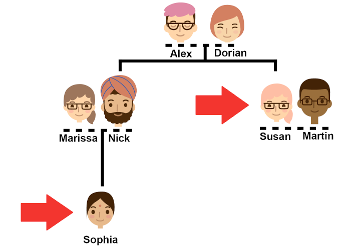
\includegraphics{pics/Sophia_Susan.png}
   
 
The shorthand notation, (first person, second person), is written when the first person is related to the second person in the Totman family tree, meaning there is a solid/half-dashed path from the first person to the second person.

We would write (Tom, Nick). But, we would not write (Tom, Marissa).  Nor would we write (Madeline, Quinn).  

The parentheses just create a nice little package of related people that is easy to read. The ordered pair tells you that there is a path, but it gives no clues about the actual path.

We now have some shorthand notation we can use when people are related. Sometimes it is appropriate (valid) to use the shorthand notation.  Like when two people are related.  Sometimes it is not appropriate (not valid).  Like when two people are not related.

Translating this into our mathematics: 

\begin{explanation}
It is appropriate to write (first person, second person) if there is a solid/half-dashed path from first person to second person that does not cross a full dashed line segment in the Totman family tree. 
\end{explanation}

\textbf{Collecting} \\
So, who is related to whom? Let's collect all of the valid pairs.  This collection will be called the Totman Relation.

(Will, Crista) is in this collection.

(Brandon, Madeline) is in this collection.

(Maegan, Lily) is not in this collection.

There are a lot of pairs in this collection and there are a lot of pairs not in this collection. The decision on membership in the collection can be determined with our science, by following paths in our picture. 








\textbf{Properties}




\textbf{QUESTION: }If (Will, Crista) is a valid pair, then is (Crista, Will) also a valid pair?

\textbf{ANSWER:} Yes. If there is a solid/half-dashed path from Will to Crista, then just follow this path backwards and you will have a valid path from Crista to Will.

In fact, this ALWAYS happens in the Totman Relation.  It is not special to Will and Crista.
If (first person, second person) is a pair in the Totman Relation, then (second person, first person) is also in the Totman Relation also, for sure, always. 


\begin{definition} 
\textbf{Symmetry} \\
When this happens for ALL pairs in a relation, we say the relation is "symmetric".  The Totman relation is symmetric.
\end{definition}



\textbf{QUESTION:} Is (Madeline, Madeline) a valid pair??

\textbf{ANSWER:} Yes There is a solid path from Madeline to Madeline, that does not cross a full dashed line segment.  It is a very very very short path, but it doesn?t include any dashes and that is the requirement.

In fact, this ALWAYS happens.  It is not special to Madeline. 

If a person is in the family tree then there is a solid path to himself or herself that does not include any full dashed line segments. (Because, you don't go anywhere.)

(person, person) is ALWAYS a pair in this relation.


\begin{definition} 
\textbf{Reflexivity} \\
When this happens for ALL items in the relation's sets, we say the relation is "reflexive".  The Totman relation is reflexive. (Note: this couldn't happen if the relation's two sets were not the same.)
\end{definition}


\textbf{QUESTION:} If (Lily, Sophia) is a valid pair, and ?(Sophia, Susan) is a valid pair, then is (Lily, Susan) also a valid pair?

\textbf{ANSWER:} No. There is a solid/half-dashed path from Lily to Sophia and a solid/half-dashed path from Sophia to Susan, but the path from Lily to Susan crosses a full dashed segment. This happens sometimes in the Totman relation and sometimes it doesn't happen.
 
 
 
 
We don't really like properties that happen sometimes. They are not as interesting as patterns that always happen.

In some relations, this ALWAYS happens for ALL of the pairs.  

If (first person, second person) is a pair in a relation and (second person, third person) is a valid pair, and that ALWAYS implies that (first person, third person) is also in the relation also, for sure, always, then we say the relation is transitive.

\begin{definition} 
\textbf{Transitivity} \\
When this happens for ALL connected pairs in the relation's sets, we say the relation is "transitive".  The Totman relation is not transitive.
\end{definition}

Whoa!  What happened there?  We are discovering more structure about our family tree.  It is further structure that our mathematics is suggesting.  This happens all the time.  

We use our science to discover structure, patterns, and relationships.  Then we describe our discoveries with our mathematics.  But, then the mathematics actually suggests more patterns and relationships that we can verify through our science. It is a never ending circle.





More Notation and Words 
The pair (James, Paula) is in the Totman relation. 
Whoa! That sentence is just too long for mathematicians. So, we have shorthand notation for "is in".  It looks like $\in$.  Kind of like a soft upper-case "E".  People might also say "is a member of" instead of "is in".  Or, "is an element of".

Inventing symbols like this happens quite often. Lots of people throughout history have thought about this stuff. Naturally, there is going to be multiple ways of saying and notating the same ideas and thoughts. - just like we experience in our everyday lives.
\textbf{COMMUNICATION} \\
The pair (Hannah, Cory) is in the Totman relation. \\
The pair (Hannah, Cory) is a member of the Totman relation. \\
(Hannah, Cory) $\in$ Totman relation \\

\begin{center}
These all say the same thing.
\end{center}






\end{document}
